A common, simple and highly used building bloc for parallel algorithms is all-prefix-sum denoted scan. Scan calculates all partial reductions of a set, as defined by Blelloch \cite{BlellochTR90} in \cref{def:al_blelloch_scan}.

\begin{definition}
\label{def:al_blelloch_scan}
\textit{The scan operation takes a binary associative operator $\oplus$, and an ordered set of n elements}
\begin{center}
$[a_0,a_1,...,a_{n-1}],$
\end{center}
\textit{and returns the ordered set}
\begin{center}
$[a_0, (a_0 \oplus a_1),...,{a_0 \oplus a_1 \oplus ... \oplus a_{a_n-1}}].$
\end{center}
\end{definition} 

The scan, like the reduction in \cref{sec:al_reduction}, is using the binary associative operator, and can therefore be used for e.g. addition or multiplication. There is distinguished between two types of scan, the exclusive scan also named prescan and the inclusive scan also just named scan. The inclusive scan is defined as \cref{def:al_blelloch_scan} where as exclusive scan is defined accordingly to Blelloch \cite{BlellochTR90} as \cref{def:al_blelloch_prescan}:

\begin{definition}
	\label{def:al_blelloch_prescan}
	\textit{The prescan operation takes a binary associative operator $\oplus$ with identity I, and an ordered set of n elements}
	\begin{center}
		$[a_0,a_1,...,a_{n-1}],$
	\end{center}
	\textit{and returns the ordered set}
	\begin{center}
		$[I,a_0, (a_0 \oplus a_1),...,{a_0 \oplus a_1 \oplus ... \oplus a_{a_n-2}}].$
	\end{center}
\end{definition} 

Both types of scan can be acquired from the other by using shifting. They are both used in different applications benefiting from there differences. Blelloch \cite{BlellochTR90} also describes the scan as a good example of an algorithm that seems inherently sequential, but for which there is an efficient parallel implementation. \Cref{fig:scan_serial} show a visual representation of the common serial implementation of the scan.  

\begin{figure}[ht]
	\centering
	\fbox{
		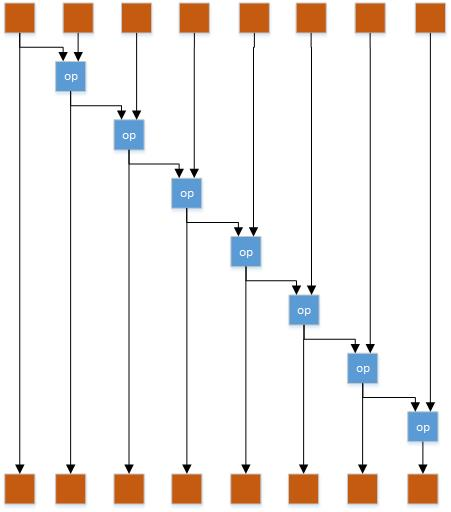
\includegraphics[width=0.4\textwidth]{figs/algorithm/scan_serial.jpg}}
	\caption{TBD}
	\label{fig:scan_serial}
\end{figure}

The algorithm looks a lot like the serial reduction on \cref{fig:reduce_serial}, but cannot be paralleled the same way because of the more strict chain of dependencies. Like the serial reduction the serial scan has a work and step complexity of O(n). The next two subsections will describe two different parallel implementations of the scan algorithm.